\documentclass{beamer}

\usetheme[progressbar=frametitle]{metropolis}
\setbeamertemplate{frame numbering}[fraction]
\useoutertheme{metropolis}
\useinnertheme{metropolis}
\usefonttheme{metropolis}
\usecolortheme{spruce}
\setbeamercolor{background canvas}{bg=white}

\usepackage{listings}
\usepackage[utf8]{inputenc}
\usepackage{enumitem}
\usepackage{caption}
\usepackage{subcaption}
\usepackage{graphicx}
\usepackage{tabularx}
\usepackage{float}
\usepackage{ragged2e}

\lstset{
    showstringspaces=false, 
    basicstyle=\ttfamily,
    tabsize=2 
}

\title{Distributed key-value store in Akka}
\date{July 28, 2020}
\author{Luca dell'Oglio}
\institute{MTDS course, Politecnico di Milano}

\begin{document}

\setcounter{framenumber}{-1}

\begin{frame}[plain]
    \titlepage
\end{frame}

\begin{frame}{Introduction} \justify

    The store has two primitives: \texttt{put(K,V)} and \texttt{get(K)}.
    
    The store should support scaling by partitioning the key-space and by assigning different keys to different nodes.

    The store should store each data element into $R$ replicas to tolerate up to $R-1$ simultaneous failures without losing any information.
    
    Upon the failure of a node, the data it stored is replicated to a new node to ensure that the system has again $R$ copies.
 
    New nodes can be added to the store dynamically.
\end{frame}

\begin{frame}{Architecture} \justify
    
    The store is implemented using the Akka clustering service. The system is composed by:

    \begin{itemize}[label=$\bullet$]
        \item Multiple \texttt{NodeActor}, which store (\texttt{key,value}) pairs;
        \item A \texttt{SupervisorActor}, which routes messages to each \texttt{NodeActor}.
    \end{itemize}

\end{frame}

\begin{frame}[fragile]{Node IDs} \justify
    
    Each node is identified by a \texttt{NodePointer}.

    \begin{lstlisting}[escapechar=\°]
class NodePointer {
    String address = node.clusterAddress;
    UInt id = hash(node.uniqueAddress);
}
    \end{lstlisting}

The same 32 bit hash function is used to obtain key IDs and node IDs.

\end{frame}

\begin{frame}{Consistent hashing} \justify

    \begin{figure}
        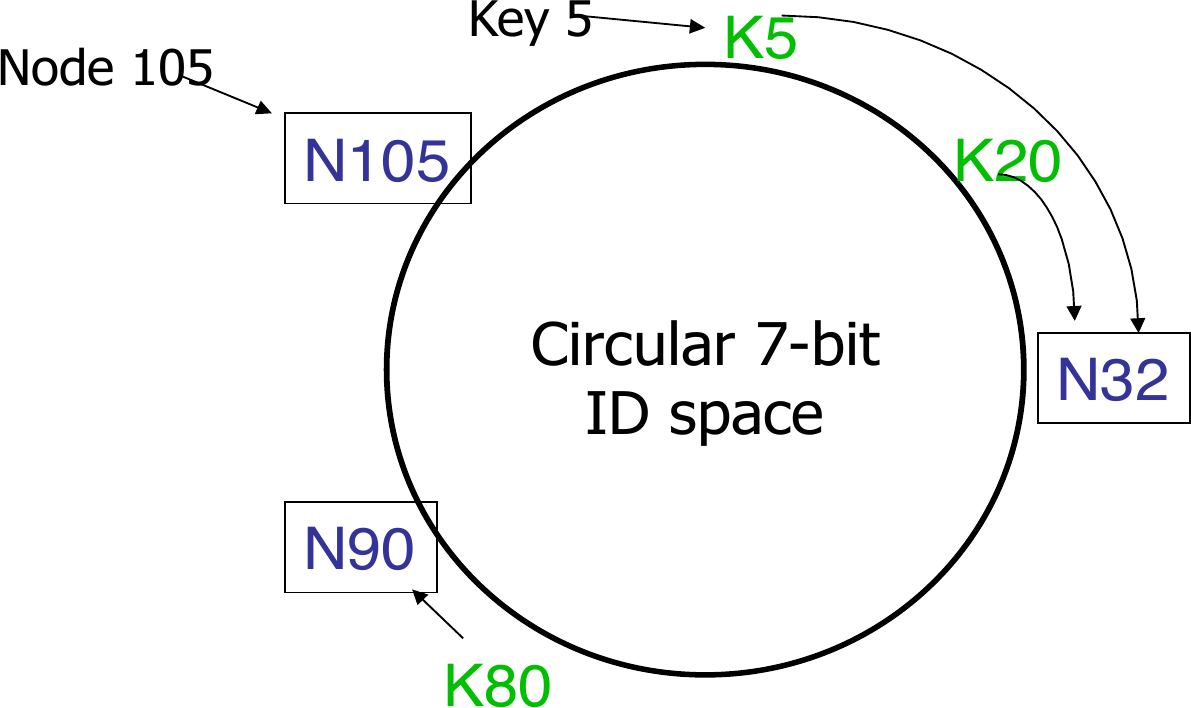
\includegraphics[width=0.5\linewidth]{00-ConsistentHashing.png}
    \end{figure}
    
    IDs are ordered on an ID ring modulo $2^m$. In this case, $m=32$.
        
    Key $k$ is assigned to the first node whose ID is equal to or follows $k$ in the identifier space. This node is called the \textit{successor node} of key $k$. 
    
    If identifiers are represented as a circle of numbers from $0$ to $2^{m - 1}$, then \texttt{succ(k)} is the first node clockwise from $k$. 

\end{frame}

\begin{frame}{Replication} \justify

    In addition to \texttt{succ(k)}, each entry (\texttt{k,v}) is stored on the $R-1$ nodes succeding the key, for a total of $R$ replicas. 

    A \texttt{get} request will try to retrieve the data from \texttt{succ(k)} first. If the request fails, it's forwarded to the next $R-1$ nodes.

    A \texttt{put} request is performed on \texttt{succ(k)}, and then the store will handle the replication separately.

\end{frame}

\begin{frame}{Implementation} \justify
    
    \texttt{SupervisorActor} stores routing information of the nodes as a \texttt{TreeSet} of \texttt{NodePointer}. The elements of the \texttt{TreeSet} are ordered in ascending order of \texttt{NodePointer.id}.

    \begin{itemize}[label=$\bullet$]
        \item Adding or removing a node and finding \texttt{succ(k)} are guaranteed to be $O(\log n)$ operations.
        \item Set elements are ordered naturally.
    \end{itemize}

\end{frame}

\begin{frame}{Node join} \justify
    When a node joins:

    \begin{itemize}[label=$\bullet$]
        \item \texttt{SupervisorActor} adds the new node to the \texttt{TreeSet};
        \item The new node receives the entries it has to store;
        \item The $R$ nodes that follow the new node clean the old keys that they don't have to store anymore. 
    \end{itemize}

    \begin{figure}
        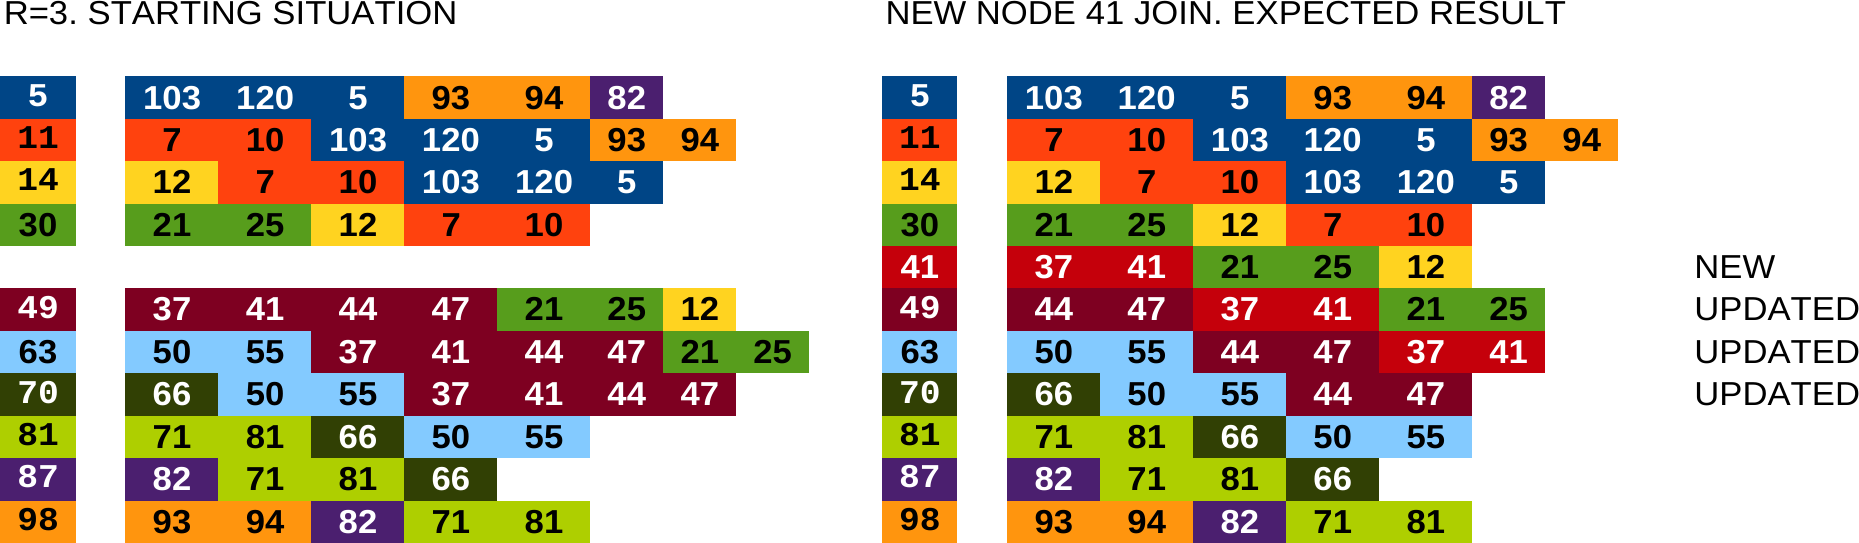
\includegraphics[width=\linewidth]{01-NodeJoin.png}
    \end{figure}
\end{frame}

\begin{frame}{Node join: new node entries (1)} \justify

    \begin{figure}
        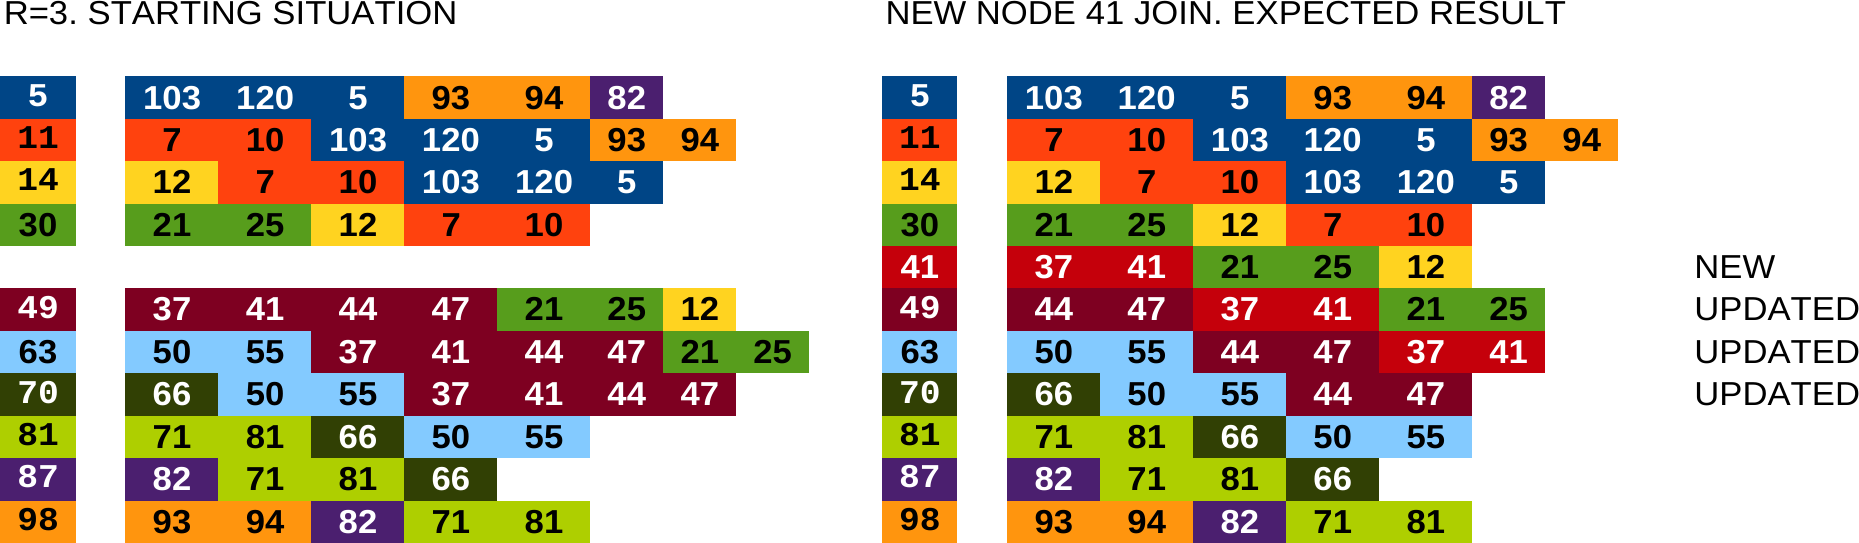
\includegraphics[width=\linewidth]{01-NodeJoin.png}
    \end{figure}

    \texttt{newNode} receives the following keys:

    \begin{itemize}[label=$\bullet$]
        \item The keys s.t. \texttt{succ(k) = newNode} from its successor (in the example, \texttt{K37, K41} from \texttt{N49});
        
        \item The replica keys from its predecessors (in the example, \texttt{K21, K25} from \texttt{N30}; and \texttt{K12} from \texttt{N14}).
    \end{itemize}

\end{frame}

\begin{frame}{Node join: new node entries (2)} \justify

    \begin{figure}
        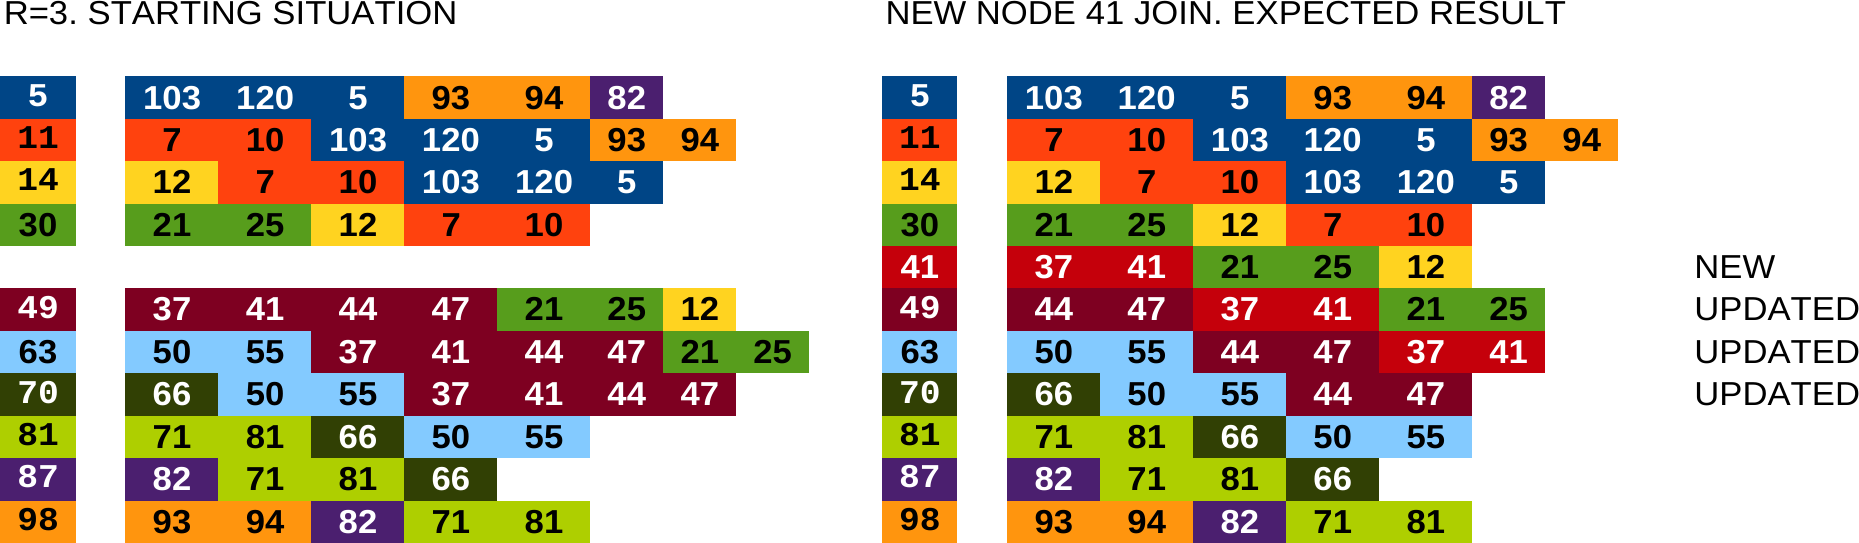
\includegraphics[width=\linewidth]{01-NodeJoin.png}
    \end{figure}

    The keys s.t. \texttt{succ(k) = newNode} from its successor (in the example, \texttt{K37, K41} from \texttt{N49}).
        
    \begin{itemize}[label=$\bullet$]
        \item \texttt{SupervisorActor} sends a \texttt{NewPredecessorMsg} to \texttt{N49}. When \texttt{N49} receives the message, it sends the required keys to \texttt{N41} (i.e., the keys for which \texttt{N41} is now directly responsible for).
    \end{itemize}

\end{frame}

\begin{frame}{Node join: new node entries (3)} \justify

    \begin{figure}
        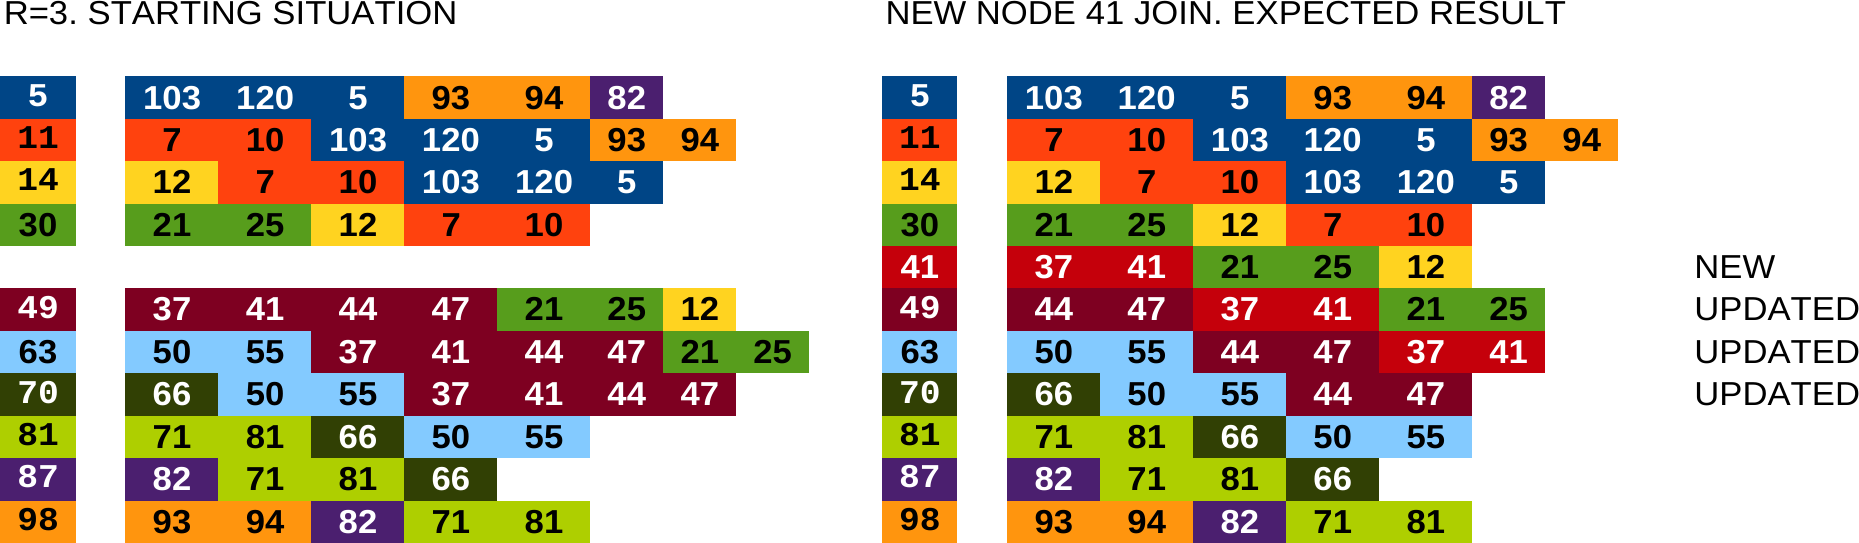
\includegraphics[width=\linewidth]{01-NodeJoin.png}
    \end{figure}

    \item The replica keys from its predecessors (in the example, \texttt{K21, K25} from \texttt{N30}; and \texttt{K12} from \texttt{N14}).

    \begin{itemize}[label=$\bullet$]
        \item See next slide.
    \end{itemize}

\end{frame}

\begin{frame}{Entries management (1)} \justify
    
    To keep the store consistent, \texttt{SupervisorActor} periodically sends each \texttt{NodeActor} two types of messages: 

    \begin{itemize}[label=$\bullet$]
        \item An \texttt{UpdateSuccessorsMsg}. When a \texttt{NodeActor} receives this message, it sends the keys for which it is directly responsible for to the first $R-1$ nodes that follows it.
        \item A \texttt{CleanKeysMsg}. When a \texttt{NodeActor} receives this message, it deletes any key that doesn't belong to its $R-1$ predecessors or for which it is not directly responsible.
    \end{itemize}

\end{frame}

\begin{frame}{Node join: new node entries (4)} \justify

    \begin{figure}
        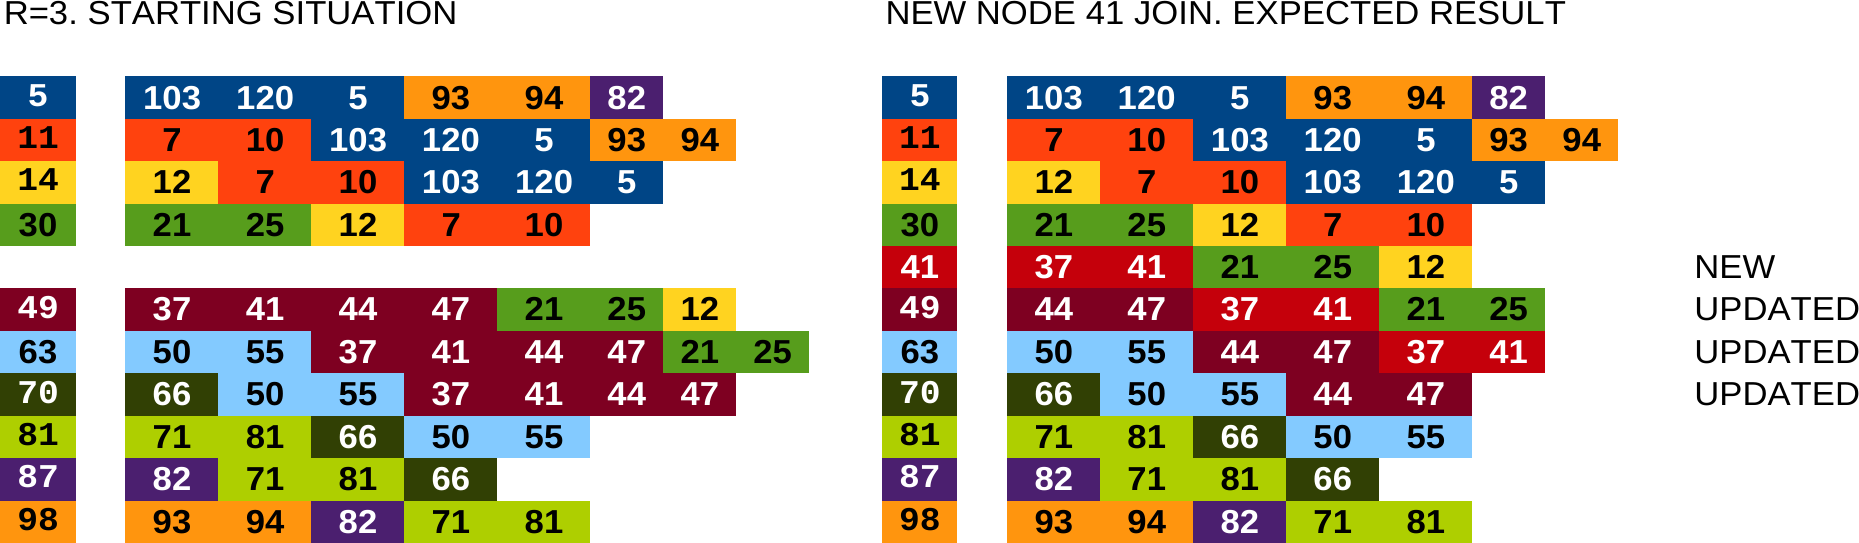
\includegraphics[width=\linewidth]{01-NodeJoin.png}
    \end{figure}

    \item The replica keys from its predecessors (in the example, \texttt{K21, K25} from \texttt{N30}; and \texttt{K12} from \texttt{N14}).

    \begin{itemize}[label=$\bullet$]
        \item An \texttt{UpdateSuccessorsMsg}. When a \texttt{NodeActor} receives this message, it sends the keys for which it is directly responsible for to the first $R-1$ nodes that follows it.
    \end{itemize}

\end{frame}

\begin{frame}{Entries management (2)} \justify

    \begin{figure}
        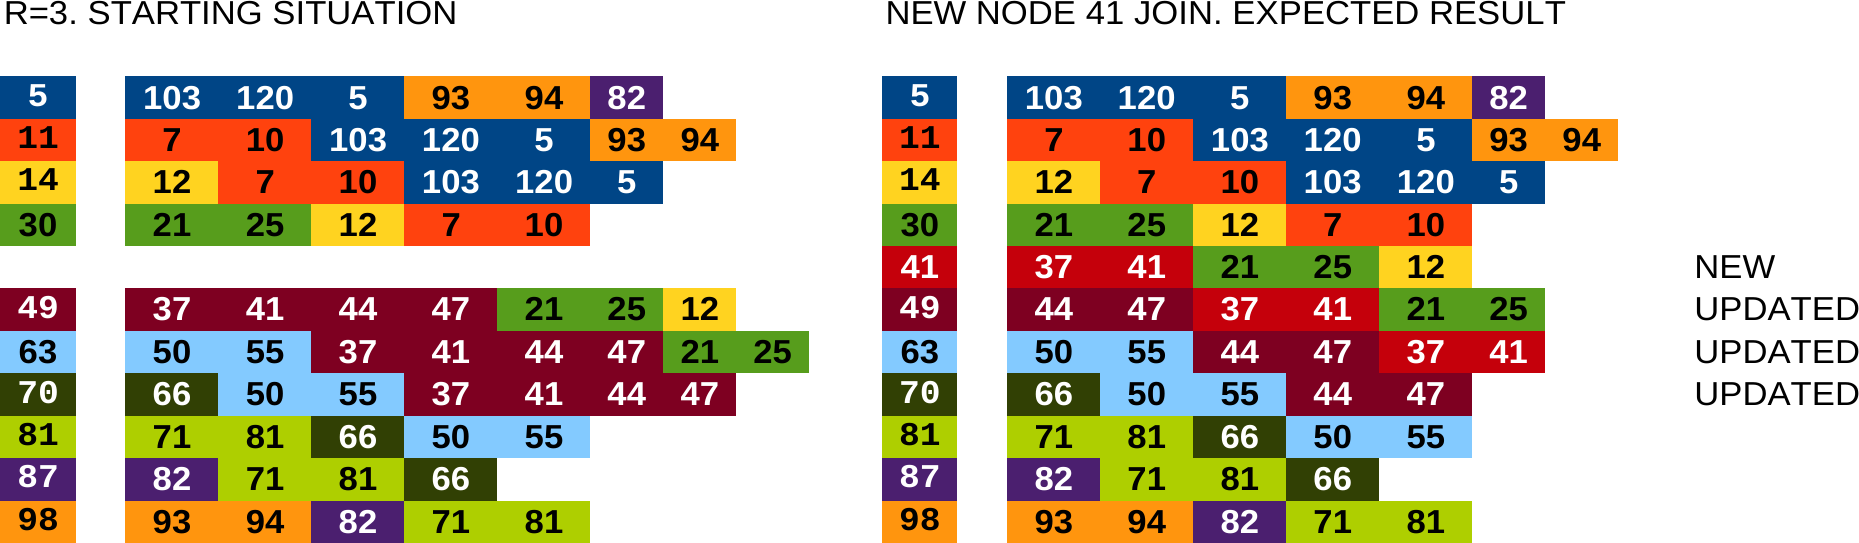
\includegraphics[width=\linewidth]{01-NodeJoin.png}
    \end{figure}

    The $R$ nodes that follow the new node clean the old keys that they don't have to store anymore. 

    \begin{itemize}[label=$\bullet$]
        \item A \texttt{CleanKeysMsg}. When a \texttt{NodeActor} receives this message, it deletes any key that doesn't belong to its $R-1$ predecessors or for which it is not directly responsible.
    \end{itemize}

\end{frame}

\begin{frame}{Node removal} \justify
    When a node is removed:

    \begin{itemize}[label=$\bullet$]
        \item \texttt{SupervisorActor} removes the new node to the \texttt{TreeSet};
        \item The store eventually becomes consistent again, thanks to the \texttt{UpdateSuccessorsMsg} messages.
    \end{itemize}

    \begin{figure}
        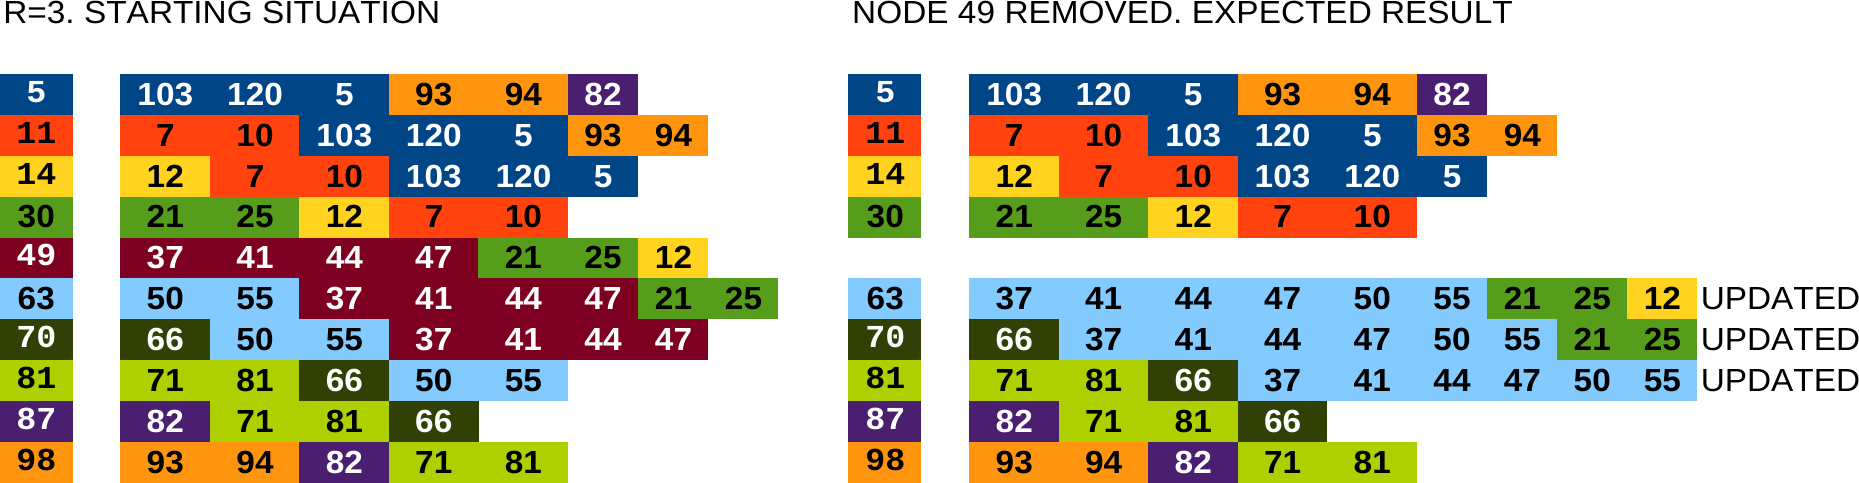
\includegraphics[width=\linewidth]{02-NodeRemoved.png}
    \end{figure}
\end{frame}



\end{document}
